\chapter{Search Engine}
Die Twitter-Klon Applikation soll mit einer Suchfunktion erweitert werden. Diese Suchfunktion wird mit einem Such-Service umgesetzt, der auf der Elasticsearch-Engine basiert. Elasticsearch setzt auf Apache Lucene auf, einer in Java geschriebenen Bibliothek für die Volltextsuche. Es ist open-source, dokumentenorientiert, in Java geschrieben und lässt sich über einen REST-API ansprechen. Damit ist es ein guter Kandidat für unser Use-Case.

\section{Zielsetzung}
Das Ziel des Suchservices ist die Ausgabe von \textit{best-match} Ranglisten über eine Tweets-Sammlung zu erstellen, indem man nach bestimmten Benutzern, Tags und Freitexteingaben sucht. Als Erweiterung der Suchfunktion wird ein Text-Vervollständigung Feature erstellt, das beim Suchen nach Tweets passende Vorschläge liefert. Und zum Schluss sollen ausgewählte Datensätze, mit Hilfe eines Analyse- und Visualisierungstools, auf der Homepage als eine Grafik angezeigt werden. 

\section{Vorgehen}
Zuerst wird eine \textit{Elasticsearch-Service} Architektur angefertigt. Diese stellt nur ein Teil der \textit{Twitter-Klon} Umsetzung und behandelt die Kommunikation zwischen \textit{Elasticsearch}, \textit{Elasticsearch-Service} wie den \textit{Kafka-Topics}. Nachfolgend wird Elasticsearch entsprechend der \textit{Twitter-Klone} Applikation konfiguriert und für die Datenaufnahmen vorbereitet. Infolgedessen wird der Such-Service implementiert, der \textit{Elasticsearch} mit den \textit{Kafka-Topics} verbindet und für den Datenaustausch zuständig ist. Anschließend werden Datenvisualisierungen mit Hilfe von \textit{Kibana} angefertigt. Zum Schluss wird der Elasticsearch Abschnitt mit einem Fazit beendet.

\section{Service Design}
Der komplette Nachrichtenaustauch der \textit{Twitter-Klon} Applikation wird mit einem skalierbaren und performanten Messaging-Service umgesetzt, nämlich \textit{Apache Kafka}. Dieser, bietet die Möglichkeit, mit Hilfe der Nachrichten-Topics den Overhead an Kommunikation zwischen den Services zu verringern, die Services von einander zu entkoppeln und die Daten parallel zu verarbeiten.
Diese Eigenschaft ermöglicht das Entkoppeln des Such-Service‘es von dem Restsystem, sodass die Suche unabhängig von den Schnittstellen der heterogenen Klienten bedient werden kann. 
Dafür wurden drei Topics erstellt und ein Datenformat vereinbart, das langfristig alle unsere Wünsche abdecken soll. Die Such-Service Use-Cases sind in drei Gruppen eingeteilt, die mit Hilfe von drei Kafka-Topics realisiert wurden: Neue Dokumente indexieren/abspeichern, Anfragen empfangen und Anfragen beantworten.
%\captionsetup{justification = raggedright,singlelinecheck = false}
\begin{figure}[htbp!]
	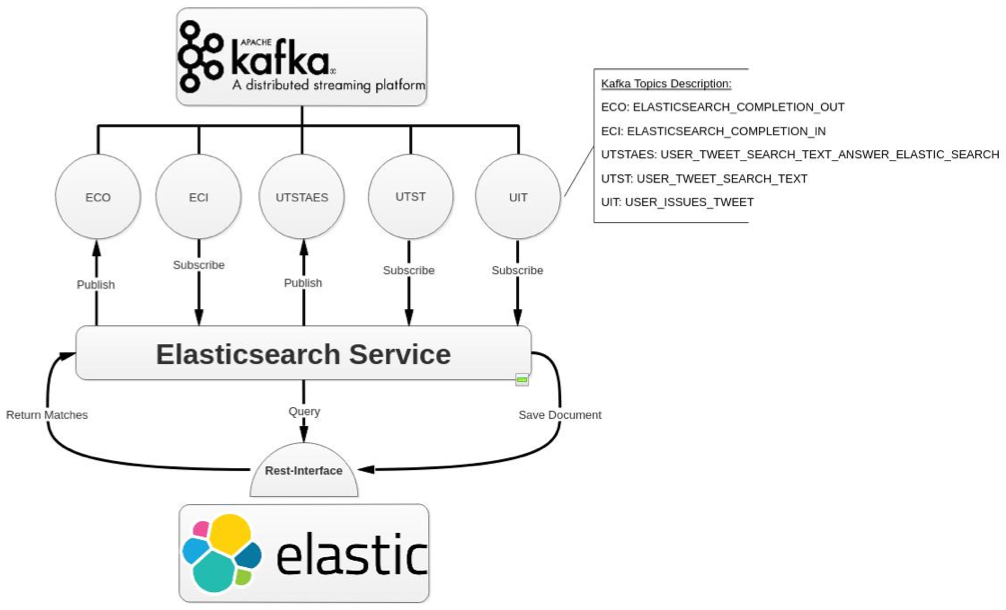
\includegraphics[scale=0.8]{material/architecture/Elasticsearch.png}
	\caption{Elasticsearch Service Architectur}
	\label{fig:ESA}
\end{figure}

Der Such-Service meldet sich an den entsprechenden Kafka-Topics an, öffnet ein Datenstrom und empfängt Nachrichten mit den Speicher-, Suchkriterien, sowie der dazugehörigen Benutzerkennung. Um den Speicherplatz optimal zu nutzen, werden aus der Nachricht nur für die Suche relevante Felder ausgelesen und an die Elasticsearch REST-Schnittstelle weitergeleitet, wie z.B. der Text, die Benutzerkennung, die Tags und der Zeitstempel.  

Das Verschicken der Nachrichten über unsere Applikation durchläuft den \textit{UIT} Topic, dieser bietet jedem Abonnenten den Zugriff auf die neu eingetroffenen Mitteilungen. Der Elasticsearch-Suchservice ist einer der bestehenden Abonnenten des \textit{UIT} Topics und bereitet die neu eingetroffenen Nachrichten für die Weiterleitung und das Speichern des Inhalts in Elasticsearch. Die, mit Metainformation bestückten, Nachrichten laufen eine Transformation durch wie Filterung, Umbenennung und Umstrukturierung, um der Elasticsearch erwarteten Datenstruktur zu entsprechen und Speicherplatz zu sparen. 

Für die Suchfunktion werden die Topics \textit{UTST} und \textit{UTSTAES} genutzt. Über den \textit{UTST} werden Suchanfragen entgegengenommen und in eine Elasticsearch-Rest-Anfrage umgeformt. Die Suchanfrage kann von dem Suchservice auf verschiedene Weise durchgeführt werden. Zum Beispiel durch eine Term-, Bollean-, Match-, Multimatch- und Match-Phrase- Suche. Jede Abfrageart, kann im bestimmten Fällen vorteilhaft ausgenutzt werden und kann Fallspezifisch eingesetzt werden. 
Das Suchergebnis wird anschließend als eine sortierte Identifikationsliste zu enthaltenen Nachrichten auf dem \textit{UTSTAES} Topic hinterlegt. Damit wäre die Suche beendet und das weitere Geschehen des Suchergebnisses den \textit{UTSTAES} Abonnenten überlassen.

Die Suchvervollständigung verhält sich ähnlich der Suchfunktion. Der Suchservice kommuniziert über die Topics \textit{ECI} und \textit{ECO}, die vervollständigung Anfragen für die Benutzereingabe publizieren und mögliche Eingabewünsche entgegennehmen. Die Eingabewünsche könne mit Hilfe der Elasticsearch Vervollständigung oder durch die nGrams-Implementation umgesetzt werden. Diese Ansätze sind in der Granularität, Umsetzung, Laufzeit und Speicherbedarf unterschiedlich und könne Fallabhängig ausgetauscht werden. 


\section{Elasticsearch Konfiguration}
Elasticsearch funktioniert \textit{out of the box}, das heißt, man muss den Service nur starten und das Indexieren, wie das Suchen der Dokumente funktioniert reibungslos. Im Gegensatz zu den relationalen Datenbanken ist eine Schema Definition für Elasticsearch nicht notwendig. Obwohl ein Schema nicht gefordert ist, ist es höchst ratsam dieses zu deferieren, denn das \textit{Type-Matching} der Felder wird ansonsten nach dem \textit{Best Guess} Prinzip erstellt und kann unter umstanden zum unerwünschten Verhalten führen.

\subsection{Index Settings}
Die \textit{out of the box} Fähigkeit von Elasticsearch ist toll zum Ausprobieren, jedoch ist es für den Betrieb ungeeignet, da die Einstellungen für die bestmögliche Skalierung von Elasticsearch, wie das Durchsuchen der Texte immer von der Domäne abhängt. Falsche oder keine Anpassung, kann die Skalierungsmöglichkeiten von Elasticsearch drastisch senken und damit den Betrieb unerwartet unterbrechen. Des Weiteren ist die Anpassung der Textvorverarbeitung eine Kernaufgabe jeder Such-Engine, dementsprechend sollte man sich besonders sorgfältig um diese Aufgabe kümmern, sodass alle relevanten Ergebnisse ermittelt und in einer passenden Ordnung dem Nutzer vorgelegt werden können.

\subsection{Sharding \& Replication}
Zuerst wird der Elasticsearch Index auf Shards und Replicas aufgeteilt. Damit enthält ein Shard eine Teilinformation oder ein Replikat der Teilinformation des Indexes, der auf unterschiedliche Hardware aufgeteilt werden kann. Obwohl die Verschiebung des Shards Knotenübergreifend realisiert werden kann, kann dieser nicht in zwei neue Shards gespalten werden, wenn die Hardware an ihre Grenzen stößt. Damit ist ein Shard die Skalierungseinheit des Indexes und muss sorgfältig gewählt werden. Der uns gegebene Elasticsearch Cluster arbeitet nur auf einem Knoten, dementsprechend ist der Skalierungsfaktor von fünf genug um zukunftssicher den Index bis auf fünf weitere Knoten aufteilen zu können. Der Replikationsfaktor beschreibt wie viele Replikate für einen Shard erstellt werden. Für eine Einstellung aus fünf Shards und einem Replikat entsteht eine Gesamtdatenmenge von 10 Shards. Daraus folgt ein immenser Anstieg an Speicherverbrauch für jeden nächsten Replikat eines Shardes. Die Replikate bieten im Gegensatz die Ausfallsicherheit und die Performance Steigerung der Lesezugriffe. Da die Performance und die Ausfallsicherheit für jeder skalierbare Applikation Kernkriterien sind, kann Elasticsearch diese bei Bedarf im laufenden Betrieb durch neue Replikate stärken. In unserem Fall steht nur einen Knoten zur Verfügung, dementsprechend folgt kein Anstieg der Performance wie Ausfallsicherheit mit Hilfe der Replikation.
% Bild  mit Reploikation der Shards und Replikas auf Knoten.
\\\\
\textbf{Initiale Index Einstellungen}
\begin{lstlisting}[language=json,firstnumber=1]
{
  "twitterindex": {
    "settings": {
      "index": {
        "number_of_shards": "2",
        "number_of_replicas": "0",
        "refresh_interval": "1s",
        "provided_name": "twitterindex",
        "creation_date": "1529674155106",
        ...
        "uuid": "wOHQnu5GQjOs7iP-Cv-_MQ",
        "version": {
          "created": "6020399"
        }
      }
    }
  }
}
\end{lstlisting}

\subsection{Textvorverarbeitung}
Als nächstes wird der Textvorverarbeitungsprozess definiert. Unter dem Schlüssel \textit{Analyzer} wird ein \textit{Custom Analyzer} und die dazugehörigen Vorverarbeitungsschritte erstellt. Dieser wird innerhalb Elasticsearch aufbewahrt und mit Funktionalität belegt. Der Analyzer zerlegt den Text mit dem \textit{Partial Word Tokenizer} in Tokens nach einem bestimmten Muster, nämlich nach einem Leerzeichen, nach einem Großbuchstaben Anfang und nach einer Zahl.
Dieser Zerlegungsschritt erfüllt die gegebenen Anforderungen, könnte aber auf Kosten des Speicherplatzes durch den mächtigeren \textit{Edge NGram Tokenizer} ausgetauscht werden. Nachfolgend laufen die Tokens eine Transformationskette durch. Zuerst werden die Tokens in Kleinbuchstaben umgewandelt, auf den Wortstamm zurückgeführt und Worte mit geringen Informationsgehalt, sowie verboten Worte entfernt. Zuletzt werden die Worte mit ähnlicher Bedeutung wie \textit{Universität Hamburg} und \textit{UHH} in Synonymlisten zusammengefasst und als gleichgültig behandelt. 
\\\\
\textbf{Analyzer}
\begin{lstlisting}[language=json,firstnumber=1]
"analyzer": {
...
  "my_analyzer": {
    "filter": [
      "my_tokenizer",
      "lowercase",
      "my_stemmer",
      "english_possessive_stemmer",
      "my_stop",
      "my_synonym"
    ],
    "type": "custom",
    "tokenizer": "standard"
  },
...
}
\end{lstlisting}

\subsection{Data Mapping}
Zuletzt braucht Elasticsearch ein Datenschema, um die automatische Fehleinschätzung des Mappings zu vermeiden. 
Elasticsearch baut einen Suchindex auf, der Dokumentenbasiert in einem JSON Format abgespeichert wird. Das Mapping garantiert eine Typenzusicherung wie das Format, der zu speichernden Felder und Dokumente. Zum Beispiel das Datumformat, das Regionsunabhängig vor dem Abspeichern von Elasticsearch normalisiert wird oder das Textfeld, das man mit bestimmten Eigenschaften und Funktionen anreichert, um das gewünschte Verhalten zu realisieren. 
Der Text, kann als \textit{Keyword} abgespeichert werden, das Eins-zu-eins durchsucht wird oder ein \textit{Text}, das mit Hilfe der Volltextsuche komplexen Suchkriterien umsetzen kann.
Das Elasticsearch Mapping für den Twitter-Klon definiert ein Dokumentenformat mit sieben Felder: id, message, tags, users, timeStamp, userLocation und userLocationCompletion. Für die Suche sind die Felder \textit{message}, \textit{tags} und \textit{use} relevant, diese werden vom Type \textit{Keyword} und \textit{Text} gespeichert. Das Feld \textit{timeStamp} wird auf ein \textit{Long} projiziert und für die Datenvisualisierung mit Kibana genutzt, um die wöchentlichen Trends anzuzeigen. Das Feld \textit{userLocation} hält die vom Benutzer eingetragene Standort, der mit der Textvervollständigungsinformation von Elasticsearch angereichert und durch das Feld \textit{userLocationCompletion} beschrieben. Zum Vergleich wird das Feld \textit{userLocation}  zusätzlich mit dem \textit{nGram Analyzer} belegt, um die Text-Verfollständigung von Elasticsearch mit der \textit{nGram} Methode vergleichen zu können.  
\\\\
\textbf{Mapping}
\begin{lstlisting}[language=json,firstnumber=1]
"userLocation": {
  "type": "text",
  "analyzer": "nGram_analyzer",
  "search_analyzer": "nGram_search_analyzer"
},
"userLocationCompletion": {
  "type": "completion",
  "analyzer": "simple",
  "preserve_separators": true,
  "preserve_position_increments": true,
  "max_input_length": 50
},
\end{lstlisting}


\section{Search Service}
Die Implementation des Such Service wird mit Java und Spring realisiert. Spring ist ein weit verbreitetes und etabliertes Enterprise Framework für Java. Dieses besitz eine große Palette an Werkzeigen, die das Arbeiten in einer heterogenen Umgebung stark vereinfachen. Daher eignet sich Spring besonders gut für unseren Anwendungsfall. Für den Nachrichtenaustausch zwischen Apache Kafka, Elasticsearch und dem Suchservice wird, die von Spring entwickelte \textit{Spring for Apache Kafka} und die von Elasticsearch angebotene \textit{Elasticsaerch Rest Client} Bibliotheken genutzt.
Die interne Logik des Suchservices wird von den Java Beans umgesetzt, die im Springkontext auf dem Apache Tomcat Application Server ausgeführt werden und die gewünschte Such-Funktionalität umsetzen.

\subsection{Such-Interface}
Um die Kommunikation und Fähigkeiten des Such Services übersichtlich zu gestalten, wird ein Interface mit den gewünschten Anfragen erstellt und anschließend implementiert. 

\begin{enumerate}
	\item über die Tags
	\item über die referenzierten Benutzer
	\item über angegebenen Standortnamen mit der Textvervollständigung
	\item über die Term-Suche auf den Tweet-Text
	\item über die Volltextsuche auf den Tweet-Text
	\item über den Text wie den Benutzet Standortnamen
	\item über einen Zeitraum
	\item über einen Zeitraum mit Benutzer und Tag Präferenz 
\end{enumerate}

\subsection{Such-Implementation}
Elasticsearch bietet eine JSON-ähnliche domänenspezifische Sprache, mit der man Abfragen ausführen kann. Dies wird als \textit{DSL Query} bezeichnet. Die Abfragesprache ist ziemlich umfassend und bietet komplexe Filter und Aggregation Möglichkeiten. Die Anfragen des Suchservices sind ausgelegt die wichtigsten Anfragemöglichkeiten von Elasticsearch darzustellen. Es werden \textit{term}, \textit{match}, \textit{multi match}, \textit{match phrase}, \textit{bool}, \textit{compleation} und \textit{aggregation} Anfragen behandelt. 
\\\\
\textbf{Suchen nach Tags}
\begin{lstlisting}[language=json,firstnumber=1]
{
  "query": {
    "terms": {
      "tags.keyword": "?"
         }
    }
}
\end{lstlisting}

\textbf{Suche nach Referenzierten Benutzer}
\begin{lstlisting}[language=json,firstnumber=1]
{
  "query": {
    "terms": {
      "users.keyword": "?"
    }
  }
}
\end{lstlisting}

Die Tag- und Benutzersuche wird mit der Term-Suche umgesetzt, diese sucht nach Dokumenten, die genau, die im angegebenen Feld angegebenen Begriffe enthalten. Die Tweets werden entsprechend den TF/IDF Relevanz sortiert und präsentiert.  
\\\\
\textbf{Textvervollständigung nach Standortnamen}
\begin{lstlisting}[language=json,firstnumber=1]
{
  "suggest": {
    "location_suggest": {
      "prefix": "?",
      "completion": {
        "field": "userLocationCompletion",
        "fuzzy": {
          "fuzziness": 1
        }
      }
    }
  }
}
\end{lstlisting}
Der Textvervollständigung bietet Funktionen zur automatischen Vervollständigung. Es werden Vorschläge wehrend des Tippens einer Anfrage getätigt und führt schneller zu relevanten Ergebnissen. Durch die zusätzliche \textit{fuzzy} Eigenschaft der Abfrage werden zusätzlich Tippfehler abgefangen um die Suche den Nutzer angenehmer zu gestalten.
\\\\
\textbf{Term-Suche auf den Tweet-Text}
\begin{lstlisting}[language=json,firstnumber=1]
{
  "query": {
    "match": {
      "message": "?"
    }
  }
}
\end{lstlisting}

\textbf{Volltextsuche auf den Tweet-Text}
\begin{lstlisting}[language=json,firstnumber=1]
{
  "query": {
    "match_phrase": {
      "message": {
        "query": "?",
        "slop": 1
      }
    }
  }
}
\end{lstlisting}

Die Suche über den Textkörper eines Tweets kann auf zwei Arten getan werden. Im ersten Fall wird eine Match-Suche \textit{metch} durchgeführt, diese normalisiert die Suchterme, verknüpft sie mit \textit{OR} und durchsucht den Textkörper nach Suchbegriff-Treffern. Im zweiten Fall nutzt man die zusammenhängende Suchanfrage \textit{phrase match}, welche im Gegensatz zu \textit{match} die Terme mit \textit{AND} verknüpft und eine Einschränkungen mitbringt, nämlich die Ordnung der Suchterme im Textkörper. Um die Suche flexibler zu gestalten, kann sie aufgeweicht werden, indem man die akzeptable Entfernung der Suchterme mit der \textit{Slope} Eingeschalt beeinflusst. In unseren Fall erlaubt diese eine Entfernung von einem Wort zwischen den Suchbegriffen.

\textbf{Standortabhängige Tweets}
 \begin{lstlisting}[language=json,firstnumber=1]
 {
  "query": {
    "multi_match": {
      "query": "?",
      "fields": [
        "message",
        "userLocation"
      ]
    }
  }
}
\end{lstlisting}

Die \textit{multi match} Abfrage sucht nach Nachrichten, dessen Inhalt einen Ort verweist und der Autor sich in dieser Region befindet. Diese Abfrage verhält sich wie \textit{match}, jedoch über eine Menge von Feldern.
\\\\
\textbf{Suche Tweets über den Zeitraum mit referenzierte Benutzer zuerst}
 \begin{lstlisting}[language=json,firstnumber=1]
{
  "query": {
    "bool": {
      "must": {
        "terms": {
          "tags": "?"
        }
      },
      "filter": {
        "range": {
          "timeStamp": {
            "gte": "now-1d/d",
            "lt": "now/d"
          }
        }
      },
      "should": [
        {
          "term": {
            "users": "?"
          }
        }
      ]
    }
  }
}
\end{lstlisting}
Diese Suchanfrage führt ein neues Konzept der \textit{bool} Anfrage, die aus mehreren Komponenten besteht. Die Suche besteht aus erforderlichen Feld-Treffern wie den optionalen Feld-Treffern. Daraus ergibt sich eine Rangordnung aus den relevanten Ergebnissen. Zuletzt läuft die Liste einen Zeitfilter durch um den Zeitraum einzuschränken. 
\\\\
\textbf{Top Tweets für die letzten sieben Tage }
 \begin{lstlisting}[language=json,firstnumber=1]
{
  "aggs": {
    "top_tags": {
      "significant_terms": {
        "field": "tags",
        "size": 10
      }
    }
  },
  "query": {
    "bool": {
      "must": [
        {
          "match_all": {}
        },
        {
          "range": {
            "timeStamp": {
              "gte": "now-7d/d",
              "lt": "now/d"
            }
          }
        }
      ]
    }
  }
}
\end{lstlisting}
Diese Anfrage ist zuständig für die Visualisierung in Kibana. In diesem Fall wird mit Hilfe der \textit{bool} Anfrage und der Elasticsearch-Aggregation, die am häufigsten verwendeten Tag über den Datensatz von sieben Tagen erarbeitet.  
\\\\
\section{Visualisierung mit Kibana}
Die Visualisierungsmöglichkeiten von Kibana sollen es ermöglichen große Datenmengen zu analysieren unterstützt durch flexible Filter. Es bietet Echtzeit-Analyse von Daten, individuell konfigurierbare Visualisierung, dynamische Dashboards und Browserbasiertes Interface, das Plattformunabhängige funktioniert.\\\\
Die Kibana Visualisierungen basieren auf den Aggregationsmöglichkeiten von Elasticsearch. Dieses aggregiert über den Elasticsearch Indexinhalt und erstellt Grafiken, die in HTML eingebunden werden können. Zur Verfügung stehende Visualisierungstypen: Area Chart, Data Table, Line Chart, Markdown Widget, Mertric, Pie Chart, Tile Map, Vertical Bar Chart.
%\captionsetup{justification = raggedright,singlelinecheck = false}
\begin{figure}[htbp!]
  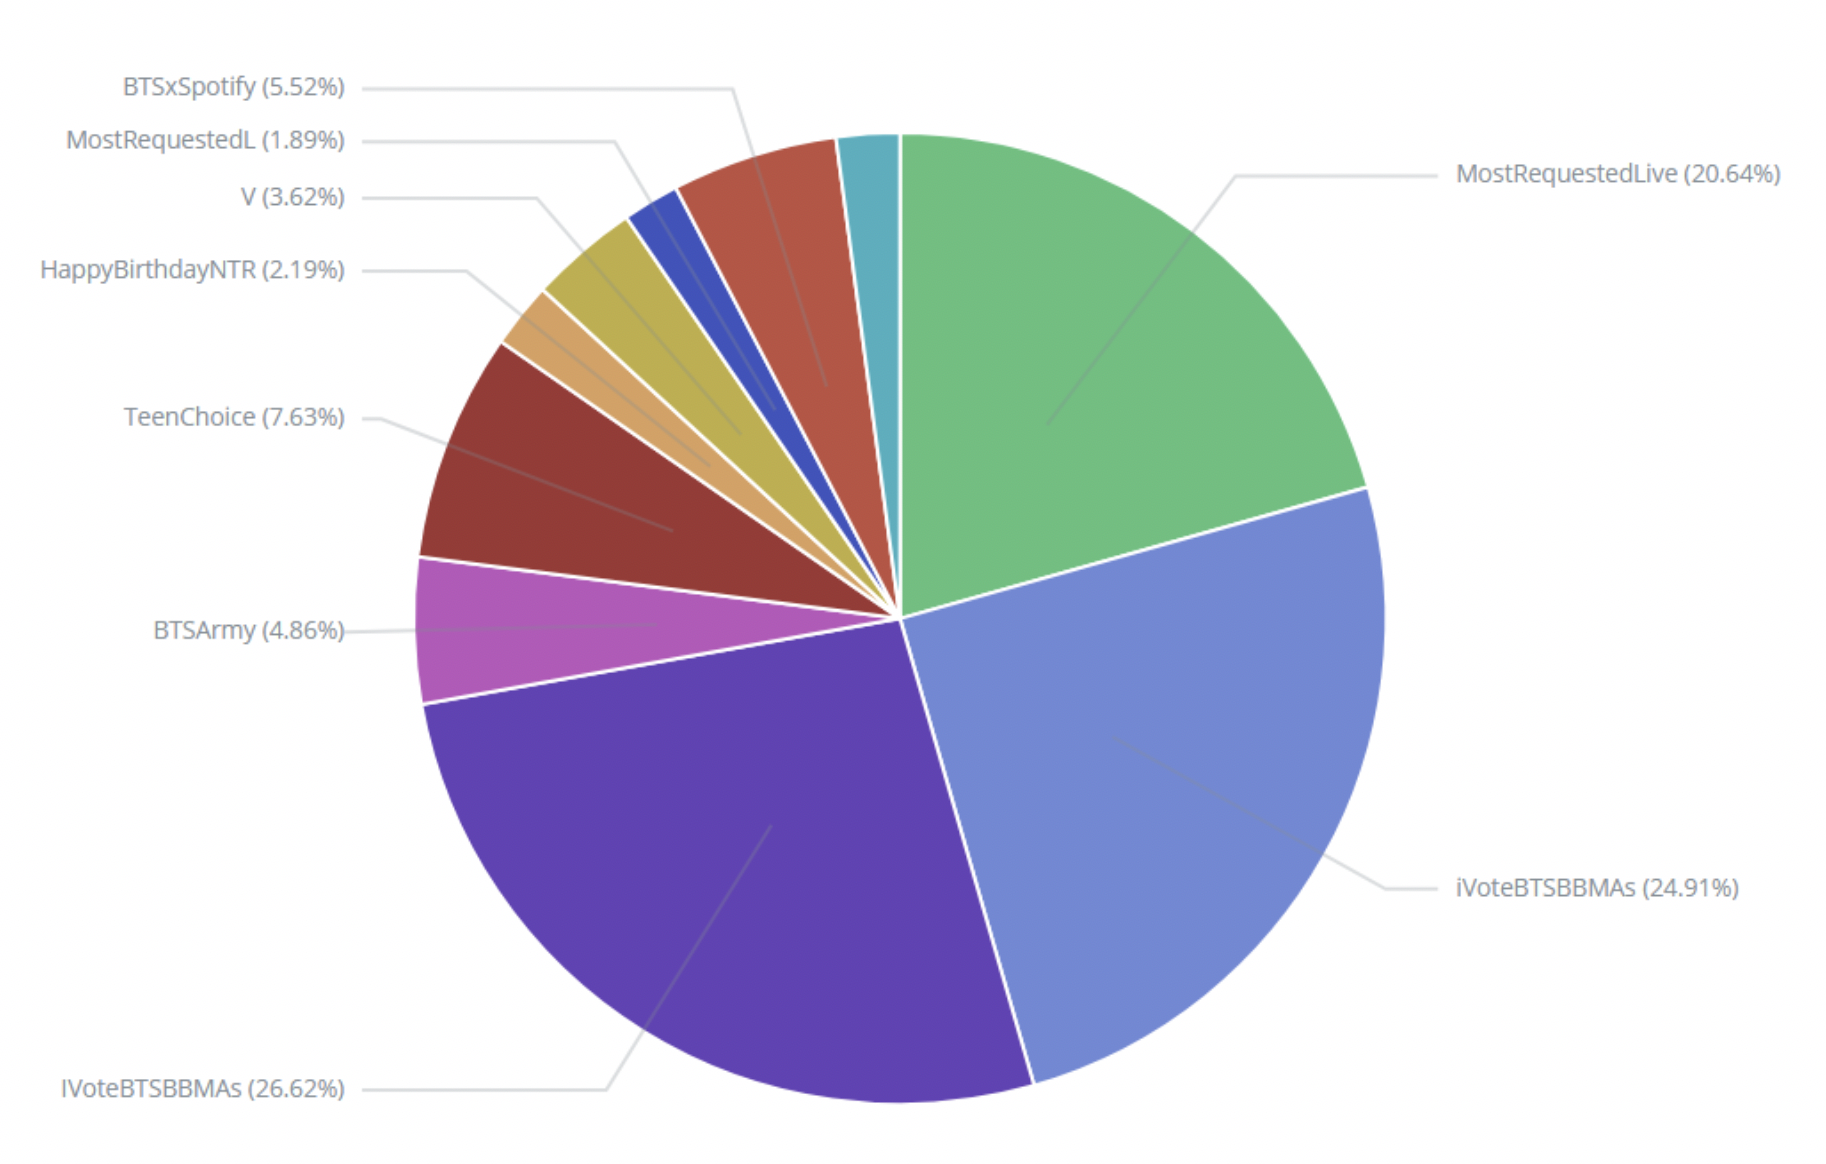
\includegraphics[scale=0.4]{material/architecture/kibana.png}
  \caption{Kibana Analyseplattform} 
  \label{fig:Kibana}
\end{figure}

\section{Fazit}
\subsection{Suchfunktionalität}
Jede moderne Software bietet eine Möglichkeit nach Daten zu suchen. Mit Hilfe von Elasticsearch kann eine einfache Suche nach einer Website oder einem Dokument innerhalb einer Sammlung implementiert werden. Anschließend kann eine Rechtschreibprüfung hinzugefügt werden. Höchstwahrscheinlich ist eine fuzzy Suche und automatische Vervollständigung nötig, möglicherweise sogar während der Eingabe. Da die Relevanz wichtig ist, können fortgeschrittene Ranking-Schemata erstellt werden. Zum Beispiel können Suchergebnisse basierend auf dem Standort, Zeit sowie des Benutzers ausgeführt werden. Und um zu wissen, was die Benutzer tatsächlich tun, kann die Nutzung der Software protokolliert und gespeichert werden für die spätere Analyse der Nutzerdaten.
\newline
Damit ist Elasticsearch eine moderne und mächtige Such-Engine, die fortgeschrittene Suchfunktionalität anbietet und für viele Anwendungsfälle geeignet ist.

\subsection{Performance}
Elasticsearch hat sich als eine robuste und fähige Such-Engine bewiesen, es konnte alle Ziele ohne Einschränkungen erfüllen und zusätzlich mit einer Vervollständigungsfunktion ergänzen. Die Index Konfiguration lässt sich einfach bedienen und über kleine Kalibrierungsschritte im JSON Format von einfachen bist komplexen Indexstrukturen erstellen. Von den Shards, Replicas bis zu den Data-Routings ist Cluster übergreifend alles möglich. Das Suchen ist eine etablierte IT-Disziplin, die mit Komfort, Kosten und Gewinn fest verbunden ist. Demgemäß ist Elasticsearch perfekt geeignet große Datenmengen zu durchsuchen und scheint mit der Anfragegeschwindigkeit, die mit jedem weiteren gefüllten Hardwareknoten die Anfragen automatisch parallelisiert. 
Somit bleibt die Geschwindigkeit im grünen Bereich auch nach dem Anstieg der Datenmenge.  
Allerdings haben die positiv gelisteten Eigenschaften ihre Tücken. Die Konfiguration des Indexes kann im Kleien so wie im Großen geschehen. Die richtige Hardware- (RAM/SSD/HDD) wie Indexkonfiguration muss gewissenhaft gewählt werden, um die versprochenen Geschwindigkeiten zu erreichen. Dementsprechend gewinnt man Zeit durch die automatisierte Datenverwaltung und verliert durch die Elasticsearch Wartung/Feinabstimmung. 

\subsection{Dokumentation und API}
Ebenso problematisch sind die Elasticsearch Abfragen, die einerseits gut im JSON-Format beschrieben und dokumentiert sind, jedoch in der Umsetzung, durch die von Elasticsearch zur Verfügung gestellten JAVA Bibliothek in JAVA schwer verständlich und Komplex in der Umsetzung.
Erst zum Ende des Projekts bin ich auf \textit{Mustach} gestoßen, die \textit{JSON-Templats} für die Abfragen erstellt und diese in einer simplen Form an Elasticsearch weiterleitet.  

\subsection{Tools}
Besondere positiv aufgefallen ist die WebUI Kibnan die mit Elasticsearch über REST Anfragen kommuniziert. Es ist möglich nach Daten zu suchen, den Clusterstatus abzufragen sowie aussagekräftige Grafiken zu erstellen. Diese Werkzeuge bieten dem Entwickler einen einfachen und übersichtlichen Einstig in die Elasticsearch-Umgebung. 

\section[Abstrakt ]{Abstrakt }



Diese Seminararbeit behandelt das Thema Informationsrückgewinnung und
soll als eine Hilfestellung, für die Umsetzung einer Such-Engine, im
„NoSQL“ Projekt dienen. 

Im Rahmen des „NoSQL“ Projektes wird eine Such-Engine benötigt, die
unstrukturierte Daten in einer Freitextform durchsucht und der Relevanz
entsprechend dem Nutzer auslegt. Um diese fachliche Anforderung zu
implementieren reicht der Key-Value Ansatz, der gängigen Datenbanken,
nicht und muss dementsprechend durch eine andere Umsetzungsform
realisiert werden. In dieser Seminararbeit werden Konzepte und
Verfahren vorgestellt, die eine Volltextsuche sowie die
Relevanzzuordnung der Suchergebnisse ermöglichen. Die entsprechende
Information kann im Buch „Introduction to Information Retrieval“ vom
Christopher D. Manning nachschlagen werden.

Die Seminararbeit beginnt mit der Abgrenzung des Begriff
„Informationsrückgewinnung“, nachfolgend gestalten Verfahren mit
Vorverarbeitungsschritten den Text durchsuchbar und zum Schluss werden
die notwendigen Schritte für die Ergebnisrangliste, der Suchanfrage,
beschrieben. 

Aufbauend auf den vorgestellten Konzepten und Verfahren wird validiert,
ob die Such-Engine {\textquotedbl}Elasticsearch{\textquotedbl} den
Projektanforderungen entspricht.




\section[Einleitung]{Einleitung}



Die zielgerichtete Suche nach Daten wird in der Regel mit einer ID-
Referenz umgesetzt und liefert ein passendes Ergebnis zu dem passenden
Schlüssel. Um eine komplizierte und erfolgreiche SQL Datenbankanfrage
durchzuführen, müssen die Daten sich in einer streng strukturierten
Form befinden. Diese Form ist passend für die Suche über Datensätze wie
Adressen, Produkte und Preise, jedoch ist sie keinesfalls für Daten
unstrukturierter Natur geeignet %
%Ohne Komma, weil kein Verb 
wie zum Beispiel die menschliche Sprache.
\newline
Die starke Entwicklung der Hardware, Software und des Internets führen
neue Informationsquellen ein: Blogs, Foren, Wikis, soziale Netzwerke
bis zu den Lernplattformen. Diese modernen Informationsquellen führen
eine große Menge an unstrukturierter Daten ein, die Durchsuchbar
gestaltet werden müssen. Damit ist die Suche über eine große Menge von
Texte in natürlicher Sprache eine zentrale Disziplin. 
\\\\
Das entschiedene Ziel der Volltextsuche: Das Auffinden und Bewerten der
relevanten Information, die in natürlicher Sprache gespeichert ist,
ohne einen Schlüsselverweis auf den enthaltenen Datensatz. 
\newline
Damit die folgende oft unangenehmen Situation nicht mehr auftritt.
\\\\
\textit{„Es tut mir leid, ich kann in Ihre Bestellung nur nachsehen, wenn Sie
mir Ihre Bestellnummer geben können.“}

\section[Begriffsklärung]{Begriffsklärung}
Der Begriff Informationsrückgewinnung kann auf unterschiedliche Weise
interpretiert und zu unterschiedlichen Disziplinen zugeordnet werden. 
\newline
Die Definition der Informationsrückgewinnung im Kontext der
Volltextsuche kann leicht missverstanden und in Verbindung mit
Datamining gebracht werden. Jedoch dürfen die beiden Disziplinen nicht
mit einander verknüpfen werden, da diese grundsätzlich unterschiedliche
Ziele verfolgen.
\newline
Die Informationsrückgewinnung soll im Gegensatz zu Datamining keine
neuen Informationen gewinnen, sondern die vorhandenen, enthaltene
Information soll zugänglich und auffindbar gemacht werden.

\section[Vorbereitung der Lösungsansätze]{Vorbereitung der Lösungsansätze}
Um die Suchansätze anschaulich darzustellen, wird ein Szenario mit einer
Sammlung von durchsuchbaren Dokument benötigt. Ein Dokument besteht aus
einer Menge von Schlüsselwertpaaren, diese können Strings, Integer und
andere Schlüsselwertpaaren enthalten. Zum Beispiel kann ein
Artikeldokument aus drei Feldern aufgebaut werden, in dem Autor, Titel
und Textkörper enthalten sind, die in sich einen beliebigen Text tragen
können (inklusive Integer, Daten, Weblinks). 
\newline
Unser Ziel ist es, aus einer Menge von Dokumenten die in sich
unterschiedliche Strukturen aufweisen dürfen, für den Nutzer relevanten
Dokumenten zu filtern.


\subsection[Lineare Suche]{Lineare Suche}
Der einfachste Weg relevante Information aus einer Datensammlung zu
filtern, ist das Scannen der Dokumente einer Sammlung nach passenden
Suchtermen und das Auslegen der Trefferdokumente als eine
Ergebnisliste. Der lineare Suchansatz kann in viele Bereichen nützlich
sein wie zum Beispiel das Linux „cat“ Funktion, jedoch ist dieser nicht
für alle Systeme und Sammlungen geeignet, denn zusammen mit der
Dokumentenanzahl wächst die Suchzeit proportional mit. 
\newline
Somit ist das Suchen in großen Datenmengen, %
%Partizip Gruppe, bezogen auf das Suchen 
besonders im Onlineformat, nicht durchführbar.

\subsection[Matrix Suche]{Matrix Suche}

Da die lineare Suche nur auf kleine Datensätze durchgeführt werden kann,
wird ein anderer Ansatz benötigt, der Arbeit im Voraus leistet, um
später die Suche zu vereinfachen. Es werden gewisse Metainformationen
des gespeicherten Dokumentes in einer Datenstruktur abgelegt, die das
Suchen unterstützen und beschleunigen sollen. 
\newline
Diese Struktur ist in einer Häufigkeitsmatrix aufgebaut und speichert
für jedes Wort und Dokument einen Boolean, der auf existieren eines
Wortes im Dokument verweist.

\begin{figure}
\centering
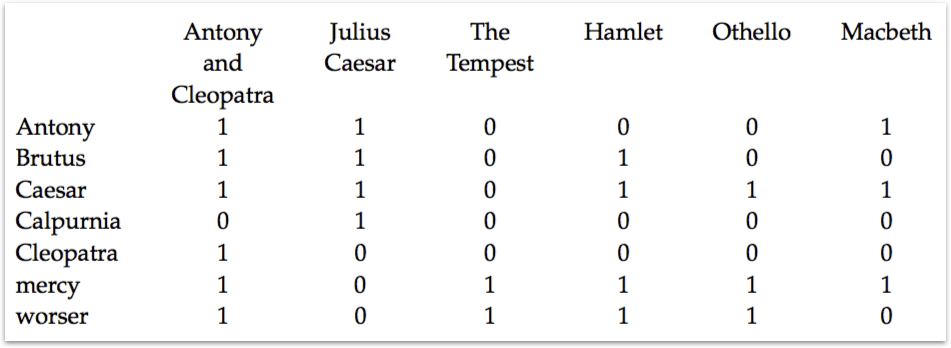
\includegraphics[width=13.54cm,height=4.955cm]{bilder/SeminararbeitArkadij-img1.png}
\caption {Häufigkeitsmatrix \cite {manning2008introduction}}
\label{manning2008introduction}
\end{figure}

\pagebreak
In dieser Datenstruktur wird die Suche in einer Boolean-Form
abgearbeitet. Es werden {\textquotedbl}1{\textquotedbl} und
{\textquotedbl}0{\textquotedbl} für jedes Dokument, das einen
bestimmten Such-Term beinhaltet, ausgelesen. Auf diese Weise können
Dokumente auf Existenz einzelner Terme untersucht werden. Ferner könne
die Terme in Kombination mit einander, durch die AND, OR, NOT
Operatoren, verarbeitet werden.
\bigbreak
Die Suche nach der Term-Kombination \textit{Brutus ${\wedge}$ Caesar ${\wedge}$
¬Calpurnia} kann jetzt leicht mit Hilfe der Häufigkeitsmatrix
berechenbar werden.
\bigbreak
\begin{center}
\textit{110100 AND 110111 AND 101111 = 100100}
\end{center}

\subsection[Invertierter Index]{Invertierter Index}
Als ein wesentlicher Nachteil der Häufigkeitsmatrix ist die dominierende
Belegung mit NULL Werten, die keine Relevanz für die Suche darstellen.
Dementsprechend gibt es einen besseren Ansatz mit Häufigkeitslisten,
die für jeden Such-Token eine Liste an Dokumentreferenzen zuweist.
Daraus entstehen auf der rechten Seite ein Wörterbuch und auf der
linken Seite eine Verweisliste. 

\begin{figure}
\centering
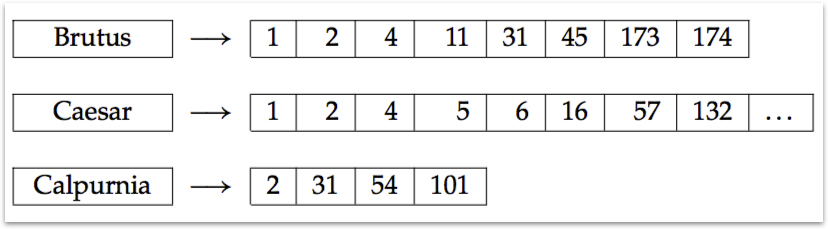
\includegraphics[width=13.143cm,height=3.634cm]{bilder/SeminararbeitArkadij-img2.png}
\caption {Häufigkeitslisten \cite {manning2008introduction}}
\end{figure}

\pagebreak 
Um die Performance der Suche zu steigern, kann die Datenstruktur in sich
geordnet aufgebaut werden, indem das Such-Term-Wörterbuch alphabetisch
und der Listeninhalt nach den Dokumenten ID’s sortiert wird. Eine
weitere Performance Steigerung ergibt sich aus der Datenstruktur, diese
erlaubt die Trennung des Wörterbuches und der Verweislisten auf
unterschiedliche Speichermedien. Dadurch wird das relativ kleine
Wörterbuch im Arbeitsspeicher gehalten und die großen Verweislisten von
der Festplatte bei Bedarf nachgeladen.

\section[Indexaufbau ]{Indexaufbau }
Bevor die Terme in den invertierten Index geladen werden, müssen diese
mehrere Vorverarbeitungsschritte durchlaufen. Die im Text vorkommende
Worte müssen in Terme aufgeteilt, gefiltert, zusammengefasst,
normalisiert und in semantisch äquivalente Gruppen zusammengefasst
werden. Erst wenn die Vorverarbeitung des Dokumentes abgearbeitet ist,
dürfen die Tokens den Index erweitern. 
\newline
Für die spätere Suche werden statistische Informationen über das
Dokument, %
%Beginn einer Erläuterung 
wie die Anzahl der Token, mitgespeichert.
\newline
Diese Informationen sind für eine Boolean-Suche nicht entscheidend,
dennoch steigern sie die Effizienz der Suchmaschine zur Abfragezeit.

\subsection[Tokenisierung]{Tokenisierung}
Im ersten Schritt wird der Text in Tokens aufgegliedert. Diese
beschreiben ein Wort oder eine Wortmenge, die einen Begriff
widerspiegeln. Dies scheint eine simple Aufgabe zu sein, jedoch hat der
Toknisierung Vorverarbeitungsschritt viele Tücken. 
\bigbreak
Namen, Nummern und Daten können von der Norm abweichende Form einnehmen
wie z.B. \textit{O'Neil}, \textit{Loas Anageles}, \textit{Mar 18,1990},
\textit{(+49)345-3455} und damit die Tokenisierung erschweren. Trotzdem müssen
die Tokens als eine Einheit erkannt und gespeichert werden. 
\newline
Zusätzlich bringt die deutsche Sprache eigne Regel, die zusätzlich beim
Tokanisieren beachtet werden müssen. Zum Beispiel muss das Wort
\textit{Lebensversicherungsgesellschaftsangestellter} in
eigenständige Einheiten zerlegt und gespeichert werden. Dieser Schritt
bedarf einer komplexen Analysephase und tiefen Verständnis der
deutschen Sprache. 
\newline
Zuletzt muss der Kontext der Datensammlung beachtet werden und die
existierenden Trends der Abkürzungen und Darstellungsformen für
bestimmte Ereignisse, Materialen, Werkzeuge und Orte miteinberechnet
werden.
\bigbreak
Demzufolge braucht der Tokenisierung-Schritt viel Aufmerksamkeit und
fein Tuning für ein angenehmes Suchverhalten. \ 

\subsection[Filterung]{Filterung}

Nachdem die Tokens gebildet wurden, kann das Filtern beginnen. Es werden
Tokens mit geringem Informationsgehalt wie \textit{der, die, das} oder in der
englischen Sprache \textit{a, an, and, are, it, be, for, let} nicht
mitgespeichert, um Ballastinformation zu vermeiden. Damit hätte man den
Speicherverbrauch stark reduziert, da diese Worte fast in jedem
Dokument in großer Anzahl auftreten werden. Allerdings können bei
diesem Sparansatz Nebeneffekte auftreten, die mit Sinn belegte Sätzen,
bestehend aus den Stoppwörtern, rausfiltern: \textit{let it be}. 

\subsection[Normalisierung ]{Normalisierung }
Im nächsten Schritt werden die Terme normalisiert. Es werden Terme mit
gleicher Bedeutung und unterschiedlicher Schreibweise zu einem Term
zusammengefasst. Zum Beispiel erwarten wir für eine Suche nach \textit{U.S.A}
ein Ergebnis, welches allen Synonymen im Text entspricht (U.S.A == USA
== United Stats of America). 
\newline
Damit die Suche Synonyme äquivalent behandelt, müssen diese mit einander
verlinkt werden. Diese Anforderung kann mit Hilfe der Äquivalenzklassen
umgesetzt werden. Sodass Begriffe die zu einer Klasse zugewiesen sind 
verallgemeinert werden und übergreifend dieselbe Bedeutung tragen.
Andererseits können Abfrageerweiterungslisten erstellt werden, die
flexibel und individuell die Bedeutung der Terme gestalten können.


\subsection[Stemming \& Lemmanisation]{Stemming \& Lemmanisation}
Die übrig gebliebenen Tokens tragen immer noch die Metainformation aus
dem Satzbau wie Zeit und Raum. Diese Information lässt einen Term mit
derselben Bedeutung unterschiedlich erscheinen, demzufolge müssen die
Terme auf eine gemeinsame Grundform zurückgeführt werden. 
\bigbreak
Es gibt zwei Ansätze dies umzusetzen. Im ersten Ansatz \texit{Lemmatisierung}
werden die Worte auf einen gemeinsamen Stamm zurückgeführt. Zum
Beispiel werden die Worte \textit{liefen, laufend, gelaufen} auf den Stamm
\textit{laufen} zurückgeführt. Dies mag eine passende Umsetzung für zahlreiche
Sprachen sein, jedoch verliert dieser Ansatz an Bindung von Worten mit
starker Ähnlichkeit wie z.B. das englische Wort \textit{operating} mit dem
Stamm \textit{operate} kann nicht auf \textit{operational} oder \textit{operative}
zurückgeführt werden. Demzufolge wird oft der \textit{Stamming} Ansatz
angewandt. Dieser trimmt die Endung eines Wortes, sodass nur die Basis
des Wortes für die Indexierung genutzt wird. Somit werden die Worte
\textit{operating} und \textit{operational} passend auf den Term \textit{operat}
runtergebrochen.

\section {Dokument Rangliste}
Bis lang wurden Konzepte der Datenstrukturen sowie der Vorverarbeitung
vorgestellt, diese bereinigen den Text vor unnötigen Information,
fassen gemeinsame Terme zusammen und speichern diese in einer für die
Suche optimalen Datenstruktur. Obwohl die Suche saubere Ergebnisse
liefert, können die Ergebnisse nicht auf Relevanz untersucht werden.
\newline
In diesem Kapitel werden die fehlenden Konzepte zur Durchführung der
Bewertung der Suchergebnisse vorgestellt.

\subsection[Dokumenten{}-Zonen]{Dokumenten-Zonen}
Das Dokument besteht aus mehreren Bereichen, diese beinhalten Terme, die
unterschiedlich gewichtet werden können, wie zum Beispiel Titel,
Textkörper und Anhang. Mit Hilfe dieser Information wird eine Ordnung
der gefundenen Dokumente erstellt und nur die wesentlichen als Ergebnis
ausgelegt.
\bigbreak
Beispielsweise wird für jeden Term ein Tupel in der Referenzliste
erstellt, das nicht nur auf das enthalte Dokument, sondern auch auf den
zugehörigen Bereich verweist. 
\bigbreak
[Willy]--{\textgreater} [2, Autor, Titel] [3, Anhang] [45, Textkörper]
\newline
\begin{wrapfigure}[7]{r}{4cm}
  \centering
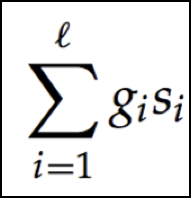
\includegraphics[width=3.381cm,height=3.507cm]{bilder/SeminararbeitArkadij-img3.png}
\end{wrapfigure}
Da die Bereiche nicht gleich wichtig sind, werden diesen Gewichte
zugewiesen, sodass sie zusammen 1 ergeben. Bei der Suche wird das
Dokument nach dem Such-Termen durchforschtet und anschließend ein
Ranking erstellt, indem die Summe der Gewichte über alle Zonen des
Dokumentes gebildet wird. 
\bigbreak
Obwohl es eine sinnvolle Umsetzung ist, mangelt dieser an Domäne Wissen
über die einzelnen Zonen, somit muss das Gewicht für jede Zone manuell
eingetragen werden. Dies ist möglich mit Hilfe eines Experten oder
einem maschinellen Lernverfahren über eine große Datenmenge, jedoch
gibt es bessere Alternativen. 

\subsection[Document Term Frequency DTF]{Document Term Frequency DTF}
Bislang wird die Bewertung eines Dokumentes über eine Term-
Existenzabfrage erstellt. In den nächsten Schritt wird diese Logik
erweitert: Ein Dokument oder eine Zone, die einen Abfragebegriff
häufiger erwähnt hat mehr mit dieser Abfrage zu tun und sollte daher
eine höhere Wertung erhalten.
\newline
Damit bekommt jeder Term in einem Dokument ein Gewichtsfaktor, der von
der Anzahl an Vorkommen von diesem Term im Dokument abhängt. Dieser
heißt \textit{Document Term Frequency} oder \textit{DTF} [tf (t,d)]. 
\newline
Für den Term „Willy“ könnte eine Referenzliste diese Form einnehmen.
\begin{center}
 [Willy]-{\textgreater} [25, Author \{6\}, Title \{25\}] [75, Title\{7\}]
\end{center}
Der vorgestellte Ansatz liefert genauere Ergebnisse, nicht desto trotz
könne die Suchergebnisse überraschen, denn nicht jedes Wort ist gleich
wichtig allen anderen Wörtern. 

\subsection[Inverse Document Frequency IDF]{Inverse Document FrequencyIDF}
Der IDF bezweckt eine bessere Bewertung des Informationsgehalts eines
Terms, denn häufig auftretende Worte innerhalb einer Sammlung haben
eine mangelhafte Aussagekraft und schränken den Suchbereich nicht ein.
Also müssen Worte, die selten auftreten, höher priorisiert werden als
Worte, die in jedem Dokument in großer Anzahl auftreten. Damit würden
oft auftretenden Terme die Suche nicht in die falsche Richtung
verzehren. 
\bigbreak
Um das geplante Verhalten zu erzeugen wird eine Formel verwendet, die
ein Verhältnis von der Gesamtheit aller Dokumente zu den Dokumenten mit
dem entsprechenden Term aufstellt.
\newline
Wenn die Gesamtzahl der Dokumente in einer Sammlung mit \textit{N} bezeichnet
wird und die Anzahl an Dokumenten, in denen ein Term \textit{t} auftaucht
\textit{DTF}, wird die inverse Dokumenthäufigkeit \textit{IDF} eines Terms \textit{t} wie
folgt definiert: 
\newline
\begin{equation*}
\scalebox{1.5}{\boxed{\mathit{IDF}\left(t\right)={\log}_{10}\left(\frac{N}{\mathit{DTF}}\right)}}
\end{equation*}
\newline
Desto weniger Dokumente mit dem entsprechenden Term in der Sammlung
existiert, desto größer der IDF und desto wichtiger die Ergebnisse.
\newline
IDF hat keine Auswirkung auf Abfragen mit einem einzelnen Term, wenn
dieser drin ist sind alle Dokumente gleichwertig.


\subsection[TF{}-IDF]{TF-IDF}
Jetzt kann die Definitionen von Dokument-Term-Häufigkeit \textit{DTF} in
gegebenen Dokument und die inversem Dokumentenhäufigkeit \textit{IDF} für den
Term kombiniert werden, um ein zusammengesetztes Gewicht für jeden Term
in jedem Dokument zu erzeugen.
\newline
Das TF-IDF-Gewichtungsschema weist dem Term \textit{t} eine Gewichtung in
Dokument \textit{d} zu, gegeben durch:
\begin{equation*}
\scalebox{1.5}{\boxed{\mathit{TF}.\mathit{IDF}=\mathit{TF}{\ast}\mathit{IDF}}}
\end{equation*}
Mit Hilfe des \textit{TF-IDF} kann das Ranking eines Dokumentes für eine gegebene
Abfrage berechnet werden. Es werden TF-IDF‘s für jeden Term, der sowohl
in der Abfrage als auch im Dokument enthalten ist, berechnet und
summiert.

Somit entsteht eine Relevanzeinschätzung für eine gegebene Abfrage und
Dokument aus der Sammlung.
\newline
\begin{figure}[h]
\centering
\scalebox{0.7}{\boxed{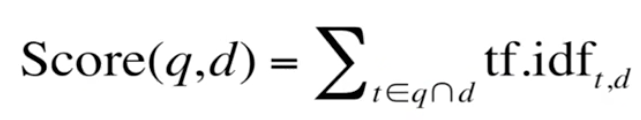
\includegraphics[width=9.821cm,height=1.838cm]{bilder/SeminararbeitArkadij-img4.png}}}
\end{figure}

Sobald für jedes Dokument der TF-IDF berechnet und in die Inzidenzmatrix
eingesetzt wurde, entsteht eine Gewichtsmatrix.

Mit Hilfe dieser, kann anhand des Dokumentenvektors ablesen werden, wie
wichtig eine Abfrage ist, indem alle vorkommen von gesuchten Termen
zusammenlegt werden.

\begin{figure}[h]
	\centering
	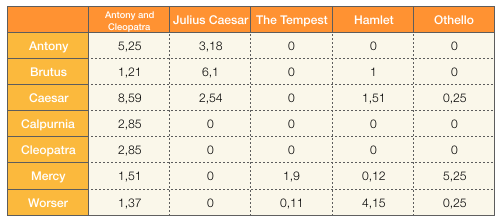
\includegraphics[width=13.208cm,height=5.854cm]{bilder/SeminararbeitArkadij-img5.png}
	\caption {TF-IDF-Matrix}
\end{figure}

\subsection[Vector Space Model ]{Vector Space Model }
Im letzten Kapitel wurden Methoden vorgestellt, wie die Dokumente in
Vektoren umgewandelt werden können, jedoch gibt es andere
Datenstrukturen, die das Erstellen des Rankings signifikant
beschleunigen können.
\newline
Das Vektormodel beschreibt ein V-Dimensionalen Vektorraum, wobei V die
Anzahl an Termen darstellt. Die Achsen des Vektorraum werden durch alle
existierenden Terme repräsentiert, die im späteren Verlauf mit der
Suchanfrage abgeglichen werden
\newline
Die Ähnlichkeit der Suchanfrage könnte über die euklidische Distanz des
Abfrage-Punkt sowie der Vektorraum-Punkte berechnet werden. Jedoch
würden Dokument, die sehr viel mit der Suchanfrage zu tun haben, sich
mit jedem Vorkommen an relevanten Termen von dem Abfrage-Punkt
entfernen. In der folgenden Abbildung besitzt ein Dokument die nötigen
Begriffe zweimal und hat damit die doppelte Entfernung vom Nullpunkt.
\begin{figure}[h]
\centering
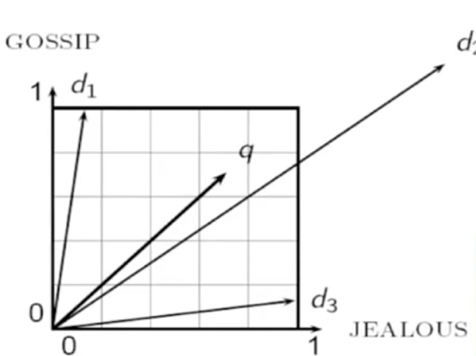
\includegraphics[width=6.435cm,height=4.81cm]{bilder/SeminararbeitArkadij-img6.png}
\caption {Euklidische Distanz \cite {manning2008introduction}}
\end{figure}
Dementsprechend sollte die euklidische Distanz nicht für die
Ähnlichkeitsberechnung der Vektoren genutzt werden und wird im
Folgenden vom winkelbasierten Ansatz abgelöst. 
\bigbreak
Beim winkelbasierten Ansatz wird die Länge der Vektoren im Vektorraum
und die Länge des Abfragevektors normalisiert und anschließend mit
Hilfe der Cosine-Similarity auf Ähnlichkeit abgeglichen.
\newline
Dabei werden Winkel zwischen der Abfrage und den Dokumenten aus der
Sammlung berechnet und Dokumente mit einer ähnlichen Ausrichtung als
Ergebnisliste zurückgegeben.
\bigbreak
\begin{figure}[H]
\centering
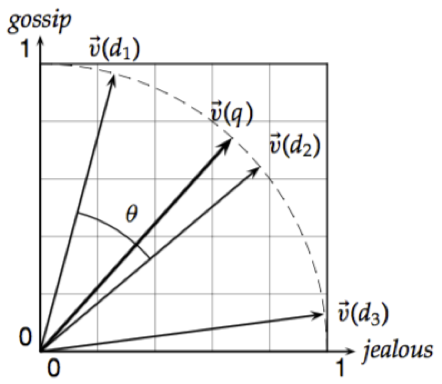
\includegraphics[width=6.361cm,height=5.528cm]{bilder/SeminararbeitArkadij-img7.png}
\caption {Winkelbasierten Ansatz \cite {manning2008introduction}}

\end{figure}
Diese Vorgehnesweise zur berechnung der Ähnlichket von zwei Vektoren
wird wie schon beschrieben durche eine Normalisierung wie Verschmelzung
der bedien Vektoren berechnet.
\newline
\begin{figure}[h]
\centering
\scalebox{1}{\boxed{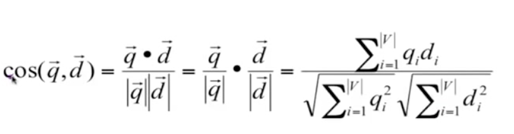
\includegraphics[width=9.465cm,height=2.466cm]{bilder/SeminararbeitArkadij-img8.png}}}
\end{figure}

\subsection[Schluss]{Schluss}
Ist eine Such-Engine die mit Volltextsuche ausgestattet ist ausreichend
für die Suche nach Textbausteinen aus einer Menge von Dokumenten? Ja,
das ist sie. Die vorgestellten Modelle zum Abspeichern von Daten in
einer Freitextform ermöglicht das Suchen nach Term-Kombinationen in
einer Datenmenge. Zusätzlich kann mit Hilfe der Metainformation des
Dokumentes wie der Sammlung Ranglisten erstellt werden, die relevante
Dokumente höher priorisieren. 
\newline
Für die Umsetzung des Datenmodells können Referenzlisten oder
Inzidenzmatrix genutzt werden.  
\newline
Für die Umsetzung der Ranglisten werden Metainformation der Sammlung,
wie der einzelner Dokumente verwendet, um bestimmte Verhältnisse
erstellen zu können.

